%!Tex Root = ../main.tex
% ./Packete.tex
% ./Design.tex
% ./Deklarationen.tex
% ./Vorbereitung.tex
% ./Aufgabe1.tex
% ./Aufgabe2.tex
% ./Aufgabe3.tex
% ./Aufgabe4.tex

\section{Bonus}

\begin{frame}[allowframebreaks]{Task \thesection}{Beweis durch Widerspruch}
  \begin{itemize}
    \item anstatt einen mathematischen Satz $S$ direkt zu beweisen, kann man seine Negation $\neg S$ durch logische Schlussfolgerungen zu einem Widerspruch führen.
    \item Wenn man die Widerspruchsanahme $\neg S$ zu einem Widerspruch geführt hat, weiß man, dass $\neg S$ immer falsch sein muss. Damit ist die doppelte Negation $\neg\neg S$ von $S$ wahr. Da $\neg\neg S \Leftrightarrow S$ eine Tautologie ist, ist $\neg\neg S$ genau dann wahr, wenn $S$ wahr ist. Damit muss $S$ wahr sein.
    \item \alert{Zerlegung der Implikation:}
    \begin{align*}
      &V o r a u s s e t z u n g_{1}\wedge\cdot\cdot\cdot\wedge\;V o r a u s s e t z u n g_{n}\rightarrow B e h a u p t u n g\\
      &\Leftrightarrow \neg\left(V o r a u s s e t z u n g_{1}\wedge\cdot\cdot\cdot\wedge\ V o r a u s s e t z u n g_{n}\right)\vee B e h a u p t u n g\\
      &\Leftrightarrow \neg\left(\left(V o r a u s s e t z u n g_{1}\wedge\cdot\cdot\cdot\wedge\;V o r a u s s e t z u n g_{n}\right)\wedge\neg B e h a u p t u n g\right)\\
      &\Leftrightarrow V o r a u s s e t z u n g_{1}\wedge\cdot\cdot\cdot\wedge\ V o r a u s s e t z u n g_{n}\wedge\lnot B e h a u p t u n g \rightarrow \perp
    \end{align*}
    \begin{itemize}
      \item \alert{Anders gesagt:} Aus den Vorraussetzungen folgt logisch die Behauptung \textit{genau dann wenn} $V o r a u s s e t z u n g_{1}\wedge\cdot\cdot\cdot\wedge\ V o r a u s s e t z u n g_{n}\wedge\lnot B e h a u p t u n g$ \textit{NICHT} gilt.
    \end{itemize}
  \end{itemize}
  \begin{Sidenote}
    \begin{itemize}
      \item es gibt neben \alert{expliziten Voraussetzungen} auch \alert{implizite Voraussetzungen}, die nicht ausdrücklich genannt werden (Rechenregeln und Standard-Definitionen)
      \item In der \alert{Behauptung} steht immer eine \alert{wahre Aussage}. Hat man eine Aussage, die \alert{nicht wahr} ist, muss man sie \alert{negiert} in die Behauptung schreiben.
    \end{itemize}
  \end{Sidenote}
  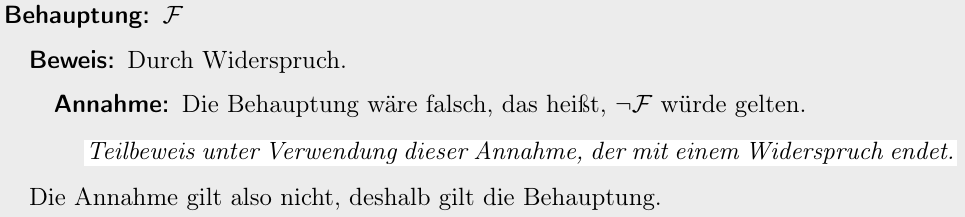
\includegraphics[width=\textwidth, center]{./figures/beweis_durch_widerspruch.png}
  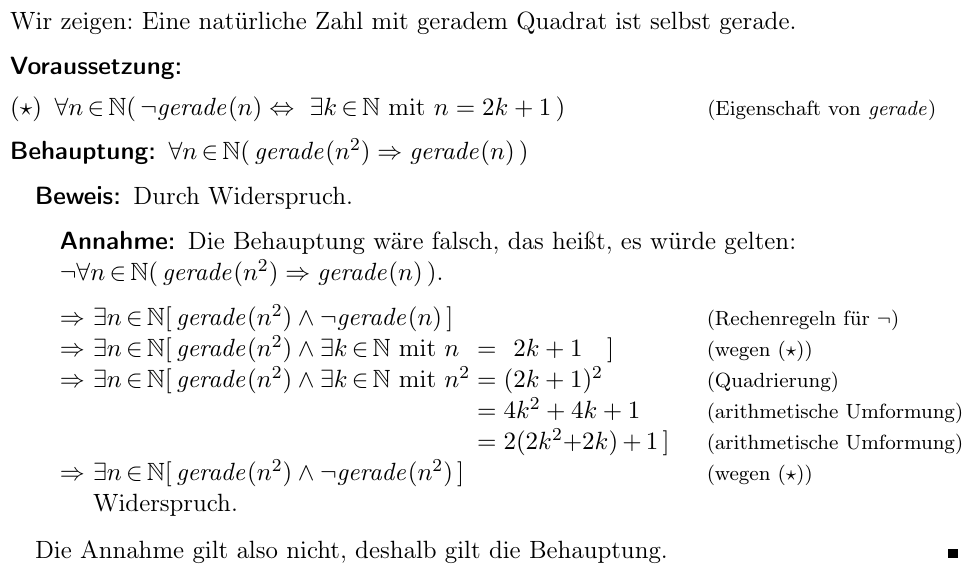
\includegraphics[width=0.7\textwidth, center]{./figures/beweis_durch_widerspruch_beispiel.png}
\end{frame}
